\documentclass[journal]{IEEEtran}
\usepackage{fancyhdr}
\usepackage{graphicx}
\usepackage[spanish]{babel}
\usepackage[utf8]{inputenc}
\usepackage{color}
\usepackage{hyperref}
\usepackage{lipsum}
\usepackage{tikz,amsmath,amssymb,amsthm,lipsum}
\usetikzlibrary{matrix}




\newcommand{\MYhead}{\smash{\scriptsize
\hfil\parbox[t][\height][t]{\textwidth}{\centering\begin{picture}(0,0) \put(-30,-13){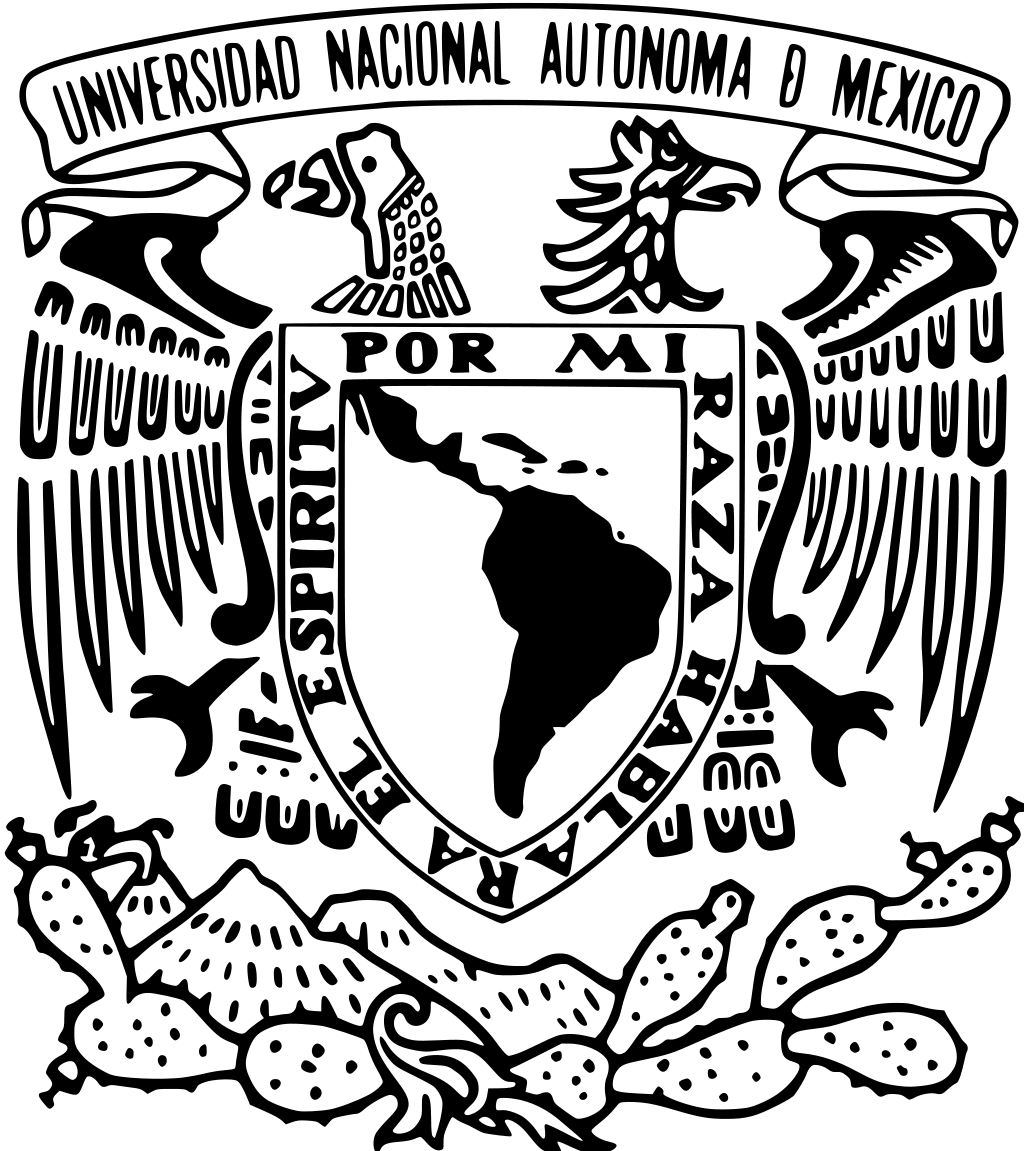
\includegraphics[width=12mm]{figs/uman.png}} \end{picture}
\hspace{7.9cm} PLANTILLA PARA PRACTICAS\\ \hspace{2cm}
\hspace{6.2cm} UNIVERSIDAD NACIONAL AUTÓNOMA DE MÉXICO \\
\underline{\hspace{ \textwidth}}}\hfil\hbox{}}}
\makeatletter


\def\ps@IEEEtitlepagestyle{%
\def\@oddhead{\MYhead}%
\def\@evenhead{\MYhead}}%
\makeatother
%______________________________________INICIO DEL DOCUMENTO________________________________%
\begin{document}

\title{Título de la práctica\\ \small{20/Nov/2022}}


\author{Perez Erick,~
        Cruz Daniel,~
        Nava Abraham,~
        y Lopez Rebeca\\
				Profesor: Pedro Arturo Flores Silva\\
\thanks{El presente documento corresponde a la práctica de [] presentado en la UNAM durante el periodo 2022-2}}


\maketitle

\begin{abstract}
\lipsum[4]
\end{abstract}

%%%%%%%%%%%%%%%%%%%%%%%%%%%%%%%%%%%%%%%%% INTRODUCCIÓN %%%%%%%%%%%%%%%%%%%%%%%%%%%%%%%%%%%%%%%%%%%%%

\section{Introducción}
\lipsum[2]

%%%%%%%%%%%%%%%%%%%%%%%%%%%%%%%%%%%%%%%%%% DESARROLLO %%%%%%%%%%%%%%%%%%%%%%%%%%%%%%%%%%%%%%%%%%%%%%

\section{Desarrollo experimental}	
\lipsum[6]

%%%%%%%%%%%%%%%%%%%%%%%%%%%%%%%%%%%%%%%%%% RESULTADOS %%%%%%%%%%%%%%%%%%%%%%%%%%%%%%%%%%%%%%%%%%%%%%

\section{Resultados y análisis de resultados}

\lipsum[5-6]
$$\lim_{x\to\infty} f(x) = (x + a) (x + b)  $$

%%%%%%%%%%%%%%%%%%%%%%%%%%%%%%%%%%%%%%%%% CONCLUSIONES %%%%%%%%%%%%%%%%%%%%%%%%%%%%%%%%%%%%%%%%%%%%%

\section{Conclusiones}
\lipsum[3]
\begin{table}[!h]
	\centering
	\begin{tabular}{|c|c|c|c|c|}
		\hline
		Mass (kg) & $\delta V \ (mV)$ & $y\ (mV)$ & $\ \varepsilon \ 10^{-3} \ $ & $ G \ \ $  \\
		\hline\hline
		0.0 & 0.01 & 0 & 0.0000 & NA\\
		\hline
		0.5 & 0.29 & 0.095 &0.0596 & 1.9475\\
		\hline
		1.0 & 0.58 & 0.184 &0.1154 &2.0110\\
		\hline
		1.5 & 0.85 & 0.273 &0.1712 &1.9863\\
		\hline
		2.0 & 1.12 & 0.361 &0.2263 &1.9793\\
		\hline
		2.5 & 1.40 & 0.450 &0.2822 &1.9848\\
		\hline
		3.0 & 1.68 & 0.540 &0.3386 &1.9848\\
		\hline
	
	\end{tabular}
	\caption{Measurement result of Exp.2}
	\label{t2}
\end{table}

%%%%%%%%%%%%%%%%%%%%%%%%%%%%%%%%%%%%%%%% BIBLIOGRAFÍA %%%%%%%%%%%%%%%%%%%%%%%%%%%%%%%%%%%%%%%%%%%%

\section{Bibliografía}

\begin{thebibliography}{1}

\bibitem{nombre_para_citar}
Inicial1.~Apellido1 and Inicial2.~Apellido2, \emph{Nombre de libro}, \#edición~ed.\hskip 1em plus
  0.5em minus 0.4em\relax Ciudad, País: Editorial, año.

\bibitem{nombre_para_citar}
Inicial1.~Apellido1 and Inicial2.~Apellido2, \emph{Nombre de libro}, \#edición~ed.\hskip 1em plus
  0.5em minus 0.4em\relax Ciudad, País: Editorial, año.

\bibitem{nombre_para_citar}
Inicial1.~Apellido1 and Inicial2.~Apellido2, \emph{Nombre de libro}, \#edición~ed.\hskip 1em plus
  0.5em minus 0.4em\relax Ciudad, País: Editorial, año.
  
\end{thebibliography}


\end{document}

%%%%%%%%%%%%%%%%%%%%%%%%%%%%%%%%%%%%%%%%%%%%%%%%%%%%%%%%%%%%%%%%%%%%%%%%%%%%%%%%%%%%%%%%%%%%%%%%%%%%